\documentclass{article}
\usepackage{amsmath}
\usepackage{graphicx}
\usepackage{listings}
\usepackage{fullpage}
\usepackage{courier}
\usepackage{float}  % Ensures figure placement

\lstset{
  basicstyle=\ttfamily\footnotesize,
  breaklines=true,
  frame=single,
}

\begin{document}

\section*{A4}

\subsection*{(a) Lasso Regularization Path}
\begin{figure}[H]
    \centering
    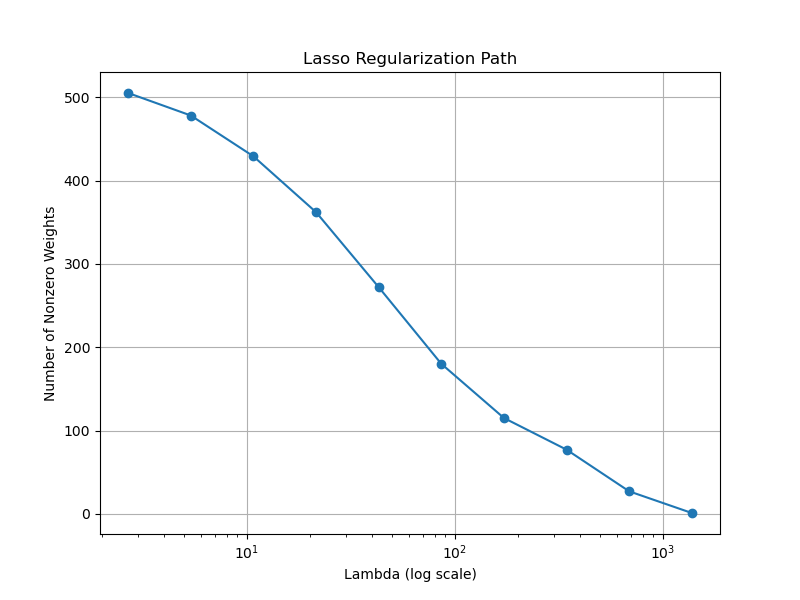
\includegraphics[width=0.6\linewidth]{C:/Users/admin/Downloads/ML/hw2/hw2/LRP.png}
    \caption{Lasso Regularization Path: Number of nonzero weights as a function of $\lambda$ on a log scale.}
    \label{fig:lasso-path}
\end{figure}

\subsection*{(b) False Discovery Rate vs. True Positive Rate}
\begin{figure}[H]
    \centering
    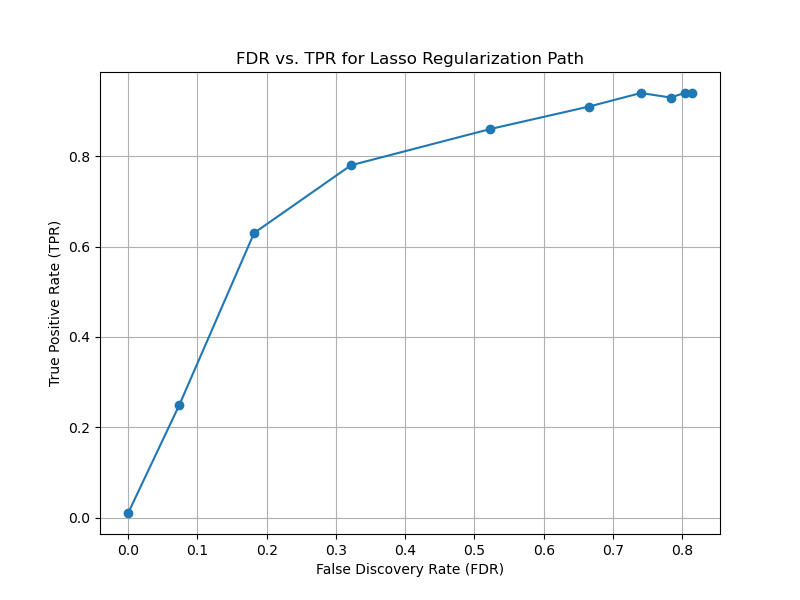
\includegraphics[width=0.6\linewidth]{C:/Users/admin/Downloads/ML/hw2/hw2/FDR_vs_TPR.png}
    \caption{FDR vs. TPR for Lasso Regularization Path. The trade-off between selecting true features and avoiding false discoveries is observed.}
    \label{fig:fdr-tpr}
\end{figure}

\subsection*{(c) Effect of $\lambda$}
As $\lambda$ increases, the Lasso penalty forces more weights to zero, leading to fewer selected features, as seen in the Lasso regularization path. In the FDR vs. TPR plot, increasing $\lambda$ initially reduces false discoveries (FDR) but at the cost of also reducing true positives (TPR), illustrating the trade-off between sparsity and correct feature selection.

\clearpage  % Forces figures to appear before the code section

\section*{Code Implementation}
\begin{lstlisting}[language=Python]
from typing import Optional, Tuple

import matplotlib.pyplot as plt
import numpy as np

from utils import problem

@problem.tag("hw2-A")
def precalculate_a(X: np.ndarray) -> np.ndarray:
    return 2 * np.sum(X ** 2, axis=0)

@problem.tag("hw2-A")
def step(
    X: np.ndarray, y: np.ndarray, weight: np.ndarray, a: np.ndarray, _lambda: float
) -> Tuple[np.ndarray, float]:
    n, d = X.shape
    residuals = y - (X @ weight)
    b = np.mean(residuals)
    for k in range(d):
        c_k = 2 * np.sum(X[:, k] * (y - (b + X @ weight + (-weight[k] * X[:, k]))))
        if c_k < -_lambda:
            weight[k] = (c_k + _lambda) / a[k]
        elif c_k > _lambda:
            weight[k] = (c_k - _lambda) / a[k]
        else:
            weight[k] = 0
    return weight, b

@problem.tag("hw2-A")
def loss(
    X: np.ndarray, y: np.ndarray, weight: np.ndarray, bias: float, _lambda: float
) -> float:
    mse = np.mean((X @ weight + bias - y) ** 2)
    l1_penalty = _lambda * np.sum(np.abs(weight))
    return mse + l1_penalty

@problem.tag("hw2-A", start_line=4)
def train(
    X: np.ndarray,
    y: np.ndarray,
    _lambda: float = 0.01,
    convergence_delta: float = 1e-4,
    start_weight: np.ndarray = None,
) -> Tuple[np.ndarray, float]:
    if start_weight is None:
        start_weight = np.zeros(X.shape[1])
    a = precalculate_a(X)
    old_w: Optional[np.ndarray] = None
    weight = np.copy(start_weight)
    while old_w is None or not convergence_criterion(weight, old_w, convergence_delta):
        old_w = np.copy(weight)
        weight, bias = step(X, y, weight, a, _lambda)
    return weight, bias

@problem.tag("hw2-A")
def convergence_criterion(
    weight: np.ndarray, old_w: np.ndarray, convergence_delta: float
) -> bool:
    return np.max(np.abs(weight - old_w)) < convergence_delta

def generate_synthetic_data(n=500, d=1000, k=100, sigma=1):
    np.random.seed(42)
    X = np.random.randn(n, d)
    X = (X - np.mean(X, axis=0)) / np.std(X, axis=0)
    true_w = np.zeros(d)
    for j in range(k):
        true_w[j] = (j + 1) / k
    epsilon = np.random.randn(n) * sigma
    y = X @ true_w + epsilon
    return X, y, true_w

def compute_lambda_max(X, y):
    y_mean = np.mean(y)
    return np.max(2 * np.abs(X.T @ (y - y_mean)))

def lasso_regularization_metrics(X, y, true_w, lambda_max, num_lambdas=10, factor=2):
    lambdas = [lambda_max / (factor ** i) for i in range(num_lambdas)]
    nonzeros = []
    fdr_values = []
    tpr_values = []

    weight = np.zeros(X.shape[1])

    for _lambda in lambdas:
        weight, _ = train(X, y, _lambda, start_weight=weight)

        nonzero_indices = np.where(weight != 0)[0]  # Features selected by Lasso
        true_nonzero_indices = np.where(true_w != 0)[0]  # True relevant features

        num_false_discoveries = np.sum(np.isin(nonzero_indices, true_nonzero_indices, invert=True))
        num_true_positives = np.sum(np.isin(nonzero_indices, true_nonzero_indices))

        total_nonzeros = len(nonzero_indices)
        fdr = num_false_discoveries / total_nonzeros if total_nonzeros > 0 else 0
        tpr = num_true_positives / len(true_nonzero_indices) if len(true_nonzero_indices) > 0 else 0

        nonzeros.append(total_nonzeros)
        fdr_values.append(fdr)
        tpr_values.append(tpr)

    return lambdas, nonzeros, fdr_values, tpr_values

def plot_lasso_path(lambdas, nonzeros):
    plt.figure(figsize=(8, 6))
    plt.plot(lambdas, nonzeros, marker='o', linestyle='-')
    plt.xscale('log')
    plt.xlabel("Lambda (log scale)")
    plt.ylabel("Number of Nonzero Weights")
    plt.title("Lasso Regularization Path")
    plt.grid(True)
    plt.show(block=False)

def plot_fdr_tpr(fdr_values, tpr_values):
    plt.figure(figsize=(8, 6))
    plt.plot(fdr_values, tpr_values, marker='o', linestyle='-')
    plt.xlabel("False Discovery Rate (FDR)")
    plt.ylabel("True Positive Rate (TPR)")
    plt.title("FDR vs. TPR for Lasso Regularization Path")
    plt.grid(True)
    plt.show()

@problem.tag("hw2-A")
def main():
    X, y, true_w = generate_synthetic_data(n=500, d=1000, k=100, sigma=1)
    lambda_max = compute_lambda_max(X, y)
    lambdas, nonzeros, fdr_values, tpr_values = lasso_regularization_metrics(X, y, true_w, lambda_max)
    plot_lasso_path(lambdas, nonzeros)
    plot_fdr_tpr(fdr_values, tpr_values)

if __name__ == "__main__":
    main()
\end{lstlisting}

\end{document}
